\documentclass[]{elsarticle} %review=doublespace preprint=single 5p=2 column
%%% Begin My package additions %%%%%%%%%%%%%%%%%%%
\usepackage[hyphens]{url}

  \journal{Geographical Analysis} % Sets Journal name


\usepackage{lineno} % add
\providecommand{\tightlist}{%
  \setlength{\itemsep}{0pt}\setlength{\parskip}{0pt}}

\usepackage{graphicx}
\usepackage{booktabs} % book-quality tables
%%%%%%%%%%%%%%%% end my additions to header

\usepackage[T1]{fontenc}
\usepackage{lmodern}
\usepackage{amssymb,amsmath}
\usepackage{ifxetex,ifluatex}
\usepackage{fixltx2e} % provides \textsubscript
% use upquote if available, for straight quotes in verbatim environments
\IfFileExists{upquote.sty}{\usepackage{upquote}}{}
\ifnum 0\ifxetex 1\fi\ifluatex 1\fi=0 % if pdftex
  \usepackage[utf8]{inputenc}
\else % if luatex or xelatex
  \usepackage{fontspec}
  \ifxetex
    \usepackage{xltxtra,xunicode}
  \fi
  \defaultfontfeatures{Mapping=tex-text,Scale=MatchLowercase}
  \newcommand{\euro}{€}
\fi
% use microtype if available
\IfFileExists{microtype.sty}{\usepackage{microtype}}{}
\bibliographystyle{elsarticle-harv}
\usepackage{graphicx}
% We will generate all images so they have a width \maxwidth. This means
% that they will get their normal width if they fit onto the page, but
% are scaled down if they would overflow the margins.
\makeatletter
\def\maxwidth{\ifdim\Gin@nat@width>\linewidth\linewidth
\else\Gin@nat@width\fi}
\makeatother
\let\Oldincludegraphics\includegraphics
\renewcommand{\includegraphics}[1]{\Oldincludegraphics[width=\maxwidth]{#1}}
\ifxetex
  \usepackage[setpagesize=false, % page size defined by xetex
              unicode=false, % unicode breaks when used with xetex
              xetex]{hyperref}
\else
  \usepackage[unicode=true]{hyperref}
\fi
\hypersetup{breaklinks=true,
            bookmarks=true,
            pdfauthor={},
            pdftitle={A spatial analysis of the environmental correlates of COVID-19 incidence in the provinces in Spain},
            colorlinks=false,
            urlcolor=blue,
            linkcolor=magenta,
            pdfborder={0 0 0}}
\urlstyle{same}  % don't use monospace font for urls

\setcounter{secnumdepth}{0}
% Pandoc toggle for numbering sections (defaults to be off)
\setcounter{secnumdepth}{0}


% Pandoc header
\usepackage{booktabs}
\usepackage{longtable}
\usepackage{array}
\usepackage{multirow}
\usepackage{wrapfig}
\usepackage{float}
\usepackage{colortbl}
\usepackage{pdflscape}
\usepackage{tabu}
\usepackage{threeparttable}
\usepackage{threeparttablex}
\usepackage[normalem]{ulem}
\usepackage{makecell}
\usepackage{xcolor}



\begin{document}
\begin{frontmatter}

  \title{A spatial analysis of the environmental correlates of COVID-19 incidence
in the provinces in Spain}
    \author[McMaster University]{Antonio Paez\corref{1}}
   \ead{paezha@mcmaster.ca} 
    \author[Universidad Politecnica de Cartagena]{Fernando A. Lopez}
   \ead{fernando.lopez@upct.es} 
    \author[Universidade Federal de Pernambuco]{Tatiane Almeida de Menezes}
   \ead{tatianedemenezes@gmail.com} 
    \author[Universidade Federal de Pernambuco]{Renata Cavalcanti}
   \ead{email@ufp.br} 
    \author[Universidade Federal de Pernambuco]{Maira Galdino da Rocha Pitta}
   \ead{email@ufp.br} 
      \address[McMaster University]{School of Geography and Earth Sciences, 1281 Main St W, Hamilton, ON,
L8S 4K1, Canada}
    \address[Universidad Politecnica de Cartagena]{Departamento de Metodos Cuantitativos, Ciencias Juridicas, y Lenguas
Modernas, Calle Real Numero 3, 30201, Cartagena, Murcia, Spain}
    \address[Universidade Federal de Pernambuco]{Departamento de Economia da Universidade Federal de Pernambuco - UFPE}
      \cortext[1]{Corresponding Author}
  
  \begin{abstract}
  Spreading with astonishing speed, the novel SARS-CoV2 has swept the
  globe, causing enormous stress to health systems and prompting social
  distance guidelines and mandates to arrest its progress. While there is
  encouraging evidence that early public health interventions have slowed
  the spread of the virus, this has come at a high cost as the global
  economy is brought to its knees. How and when to ease restrictions to
  movement hinges in part on the question whether SARS-CoV2 will display
  seasonality associated with variations in temperature and humidity. In
  this research, we address this question by means of a spatial analysis
  of the incidence of COVID-19 in the provinces in Spain. Use of a spatial
  SUR approach allows us to model the incidence of reported cases of the
  disease per 100,000 population, as a function of temperature and
  humidity, while controlling for GDP per capita, population density,
  percentage of older adults in the population, and presence of mass
  transit systems. Our results indicate that incidence of the disease is
  lower at higher temperatures. The evidence with respect to humidity is
  more mixed, with coefficients for this variable that are significant in
  only some equations. Our control variables also yield interesting
  insights, as population density and percentage of older adults display
  negative associations with incidence of COVID-19, whereas the presence
  of mass transit systems in the province is associated with a greater
  incidence of the disease.
  \end{abstract}
  
 \end{frontmatter}

\hypertarget{introduction}{%
\section{Introduction}\label{introduction}}

From a small outbreak linked to a live animal market at the end of 2019
to a global pandemic in a matter of weeks, the SARS-CoV2 virus has
threatened to overrun health systems the world over. In efforts to
contain the spread, numerous governments in many nations and regions
have either recommended or mandated social distancing measures, and as
of this writing, millions of people in five continents shelter in place.
There are encouraging signs that these measures have arrested the spread
of the virus where they have been implemented, and have thus helped to
keep a bad situation from becoming even worse (e.g., 2020). However,
this has come at a high cost, and the consequences for all spheres of
the economy, social, and cultural life have been dire (e.g., Fernandes,
2020; Luo and Tsang, 2020). As a result, there is a sense of urgency to
anticipate the progression of the pandemic, in order to plan for
progressive lifting of restrictions to movement and social contact
(e.g., Kissler et al., 2020). Needless to say, this has become a
delicate, and politically charged, balancing act between public health
and the economy (Gong et al., 2020).

A salient question in the debate on how and when to ease social
distancing measures is whether the virus will display seasonal
variations. Earlier, diverse studies have shown the effect of
temperature and humidity on the incidence of influenza (e.g., Mäkainen
et al., 2009; Jaakkola et al., 2014; Kudo et al., 2019). Jaakkola et
al.~(2014), for example, found that a decrease of temperature and
absolute humidity precedes the onset of symptoms of influenza A and B
viruses by 3 days in places where the temperature is low. After the
2002-2004 outbreak of SARS, researchers also began to investigate the
relationship between these factors and SARS-CoV. In this way, Casanova
et al.~(2010) used two surrogates, namely the gastroenteritis (TGEV) and
mouse hepatitis viruses (MHV), to find that virus inactivation was more
rapid at temperatures of 20C than 4C, and at 40C than 20C; in terms of
humidity, these researchers reported that survival of the virus was
lower at moderate relative humidity levels. In a similar vein, but
working directly with SARS-CoV, Chan et al.~(2011) found that viability
of the virus was lost at temperatures higher than 38C and relative
humidity superior to 95\%.

While existing research on similar pathogens suggests that SARS-CoV is
more stable and potentially easier to transmit in conditions of low
temperature and low humidity, it is far from certain that this will also
be the case with the novel SARS-CoV2. If such is the case, there is the
possibility of easing restrictions to social contact as the weather
warms; however, weeks or possibly months of costly measures could become
undone if not, and the restrictions are lifted prematurely. Not
surprisingly, this issue has triggered a lively debate.

In this paper, we report results from a spatial analysis of incidence of
COVID-19 in fifty provinces in Spain. Spain is one of the countries
hardest hit by the virus, and enacted lockdown measures on March 16,
2020, in response to a rapidly growing outbreak of COVID-19. We combine
data on reported cases of the disease with metereological information,
to create a spatio-temporal dataset covering a period of 30 days. We
then join this dataset with provincial-level economic and demographic
information to act as controls to our key environmental variables. These
data are analyzed using a spatial SUR approach, which allows us to
account for residual spatial autocorrelation.

The results provide persuasive evidence of the effect of temperature on
the incidence of COVID-19, as \textbf{NOTE ABOUT THE MAGNITUDE OF THE
EFFECT}. The evidence concerning humidity is more mixed: while the
direction of the effect is negative, as anticipated, the coefficients
for this variable are only significant in some of equations in the
system. Our control variables also provide some intriguing insights. The
results of this analysis provide support to the hypothesis of
seasonality of the novel SARS-CoV2, and should be of interest to public
health officials and policy makers wrestling with the question of the
trajectory of the pandemic.

Please note that this paper is prepared as a reproducible research
document. The source R Markdown document, as well as all data and code
needed to reproduce/review/extend the analysis can be obtained from the
following repository:

\begin{quote}
\begin{quote}
Include link to repository
\end{quote}
\end{quote}

\hypertarget{context-and-data}{%
\section{Context and Data}\label{context-and-data}}

\hypertarget{covid-19-in-spain}{%
\subsection{Covid-19 in Spain}\label{covid-19-in-spain}}

When was the first case reported? When did the country close
international arrivals? When did initial measures of social distancing
were implemented? The lockdown?

\hypertarget{selection-of-variables}{%
\subsection{Selection of Variables}\label{selection-of-variables}}

Explain the rationale for selecting the variables.

\hypertarget{sources-of-data-and-data-preparation}{%
\subsection{Sources of Data and Data
Preparation}\label{sources-of-data-and-data-preparation}}

Explain the sources of data and data preprocessing.

Descriptive statistics of the incidence of COVID-19 and provincial
economic and demographic variables are shown in Table
\ref{tab:descriptive-statistics}.

\begin{table}

\caption{\label{tab:descriptive-statistics}\label{tab:descriptive-statistics}Descriptive statistics}
\centering
\resizebox{\linewidth}{!}{
\begin{tabular}[t]{l>{\raggedright\arraybackslash}p{15em}rrrr>{\raggedright\arraybackslash}p{15em}}
\toprule
Variable & Note & Min & Mean & Max & SD & Source\\
\midrule
\rowcolor{gray!6}  SARS-19 Incidence & Incidence in reported cases of SARS-19 per 100,000 people & 0.38 & 153.61 & 1149.36 & 186.23 & Source\\
GDPpc & GDP per capita in €1,000s & 16.67 & 22.51 & 36.00 & 4.77 & Source\\
\rowcolor{gray!6}  Older & Percentage of people aged 65 and older in the province & 15.16 & 21.03 & 31.36 & 3.95 & Source\\
Population Density & Population density in the province in people per sq.km & 8.60 & 140.04 & 829.76 & 181.25 & Source\\
\bottomrule
\end{tabular}}
\end{table}

\begin{figure}
\centering
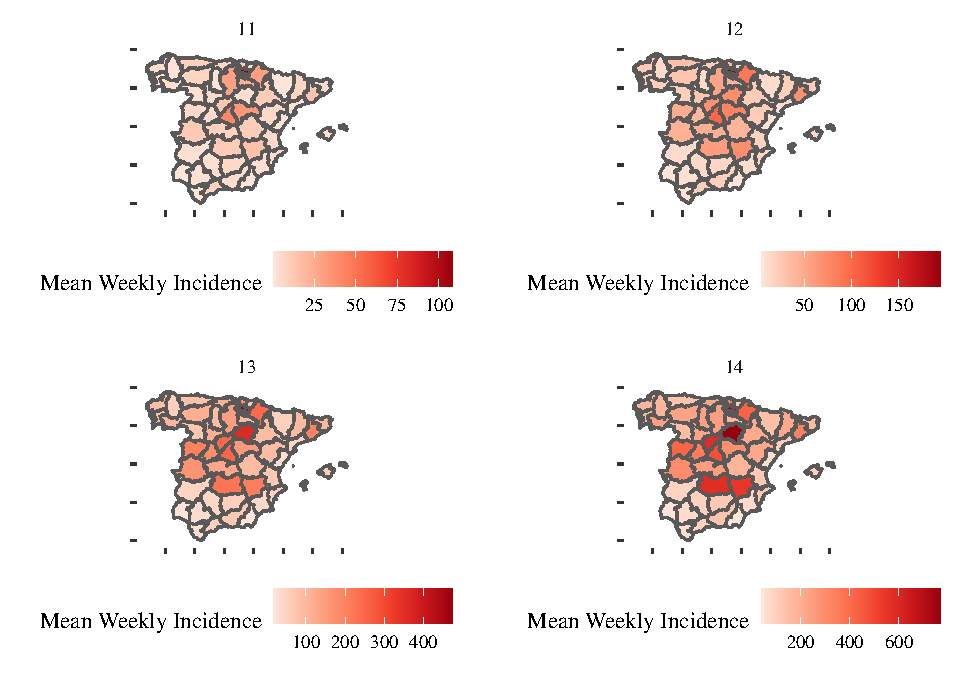
\includegraphics{Climatic-Correlates-of-COVID19-Spain_files/figure-latex/weekly-average-incidence-map-1.pdf}
\caption{\{fig:weekly-average-incidence-map\}Mean weekly incidence of
COVID-19 by province, in reported cases by 100,000 people}
\end{figure}

\begin{figure}
\centering
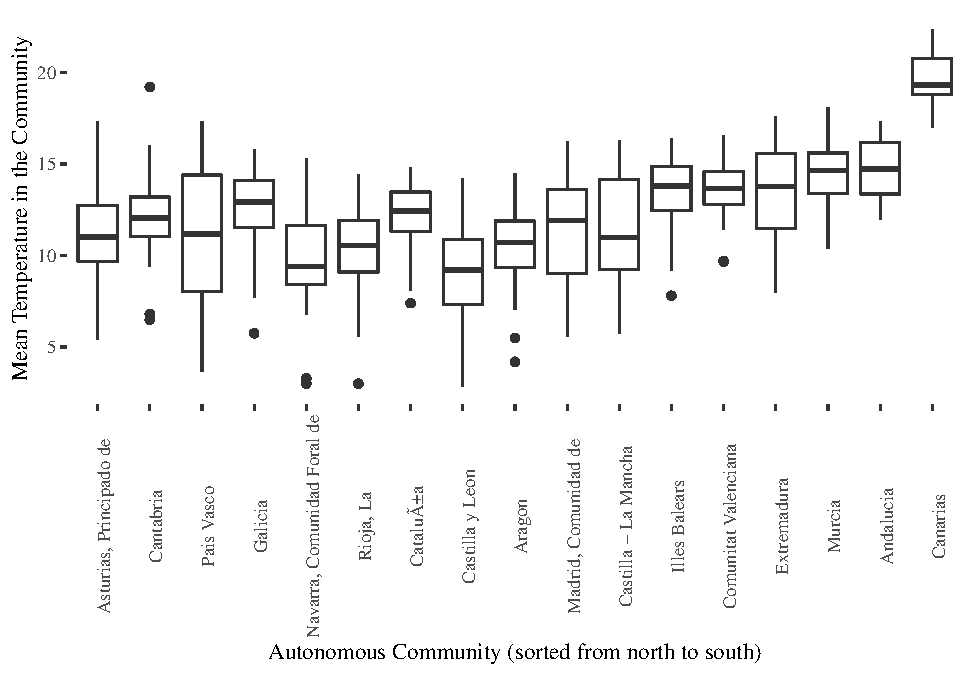
\includegraphics{Climatic-Correlates-of-COVID19-Spain_files/figure-latex/descriptives-temperature-1.pdf}
\caption{\label{fig:descriptives-temperature} Distribution of
temperatures in the Autonomous Communities in Spain between March 12,
2020 and April 11, 2020. The Autonomous Communities have been sorted by
latitude, with communities to the left being the northermost, and to the
right the southernmost}
\end{figure}

\begin{figure}
\centering
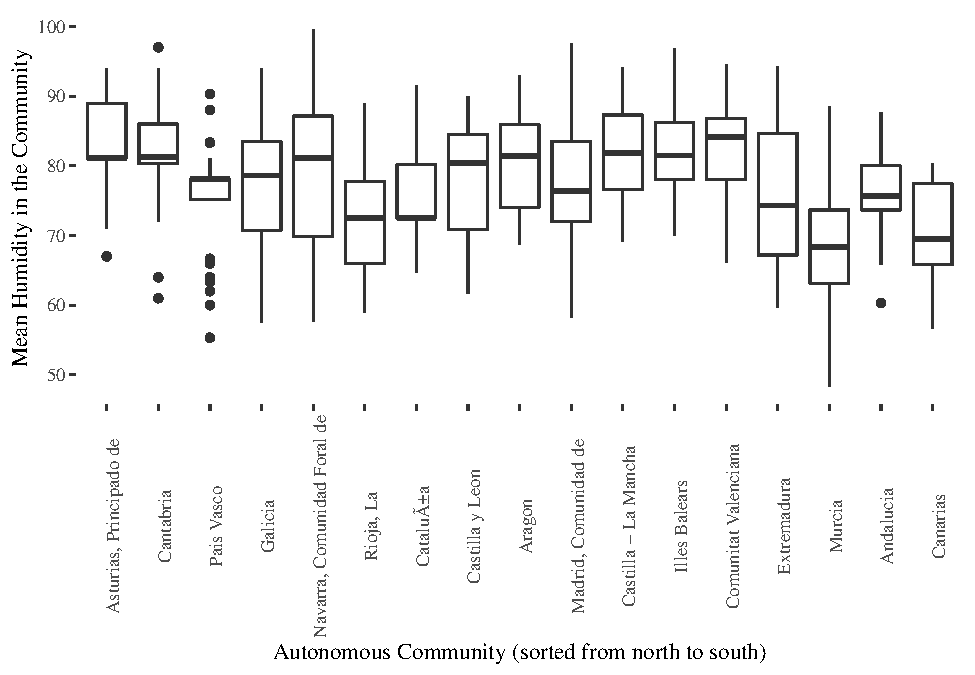
\includegraphics{Climatic-Correlates-of-COVID19-Spain_files/figure-latex/descriptives-humidity-1.pdf}
\caption{\label{fig:descriptives-humidity} Distribution of humidity in
the Autonomous Communities in Spain between March 12, 2020 and April 11,
2020. The Autonomous Communities have been sorted by latitude, with
communities to the left being the northermost, and to the right the
southernmost}
\end{figure}

\hypertarget{methods-spatial-sur}{%
\section{Methods: Spatial SUR}\label{methods-spatial-sur}}

\hypertarget{the-econometric-model}{%
\section{The econometric model}\label{the-econometric-model}}

The baseline model propouse in this paper is a classical SUR model
without spatial effects (from here, SUR-SIM). Following the classical
expresion for thios model in stacked form

\begin{equation}
\begin{bmatrix}
y_1 \\ y_2 \\ ... \\ y_T
\end{bmatrix}
=
\begin{bmatrix}
X_1 & 0 & ... & 0 \\ 0 & X_2 & ... & 0 \\ ... & ... & ... & ... \\ 0 & 0 & ... & X_T
\end{bmatrix}
\
\begin{bmatrix}
\beta_1 \\ \beta_1 \\ ... \\ \beta_T
\end{bmatrix}
+
\begin{bmatrix}
\epsilon_1 \\ \epsilon_2 \\ ... \\ \epsilon_T
\end{bmatrix}
\label{eq:sur-sim}
\end{equation}

where \(y_{t}=(y_{1t},...,y_{Nt})\) is the incidence ratio in the
province \(s\) (\(s=1,...,N\)) the day \(t\) \((t=1,...,T)\); \(X_t\) is
a \(N \times k_t\) matrix of the \(k_t\) independen variables;
\(\beta_t=(\beta_{1t},...,\beta_{Nt})\) is a vector of coefficients and
\(\epsilon\) is the error vector. Like is characteristic in SUR model,
we consider dependence among error vector
\(E[\epsilon_t \epsilon'_{t'}]=\sigma_{tt'}]\). Note that this
especification is flexible allowing changes in the coefficients
\(\beta_{it}\) in order to modulate the effect of \(X_it\) on \(y_t\).
This flexibility is not always diserable and is posible impose
restrinctions and consider time constant some \(\beta\) coefficients. In
this case we can reformulate the coefficients expression of
\(\beta_t=(\beta_{1},...,\beta_{r},\beta_{r+1},...,\beta_{Nt})\) if we
want to consider the first \(r\) coefficients contanst. The equation
({\textbf{???}})\{eq:sur-sim\} can be write in compact form,
\begin{equation}
y = X \beta + \epsilon
\end{equation} where\ldots.

Like in case of cross-section, it is possible identify spatial
autocorrelation in the residuals of ({\textbf{???}})\{eq:sur-sim\} and
several tests has been develop to test the null of spatial independence
(López Mur Herrera). In case of reject the null alternative
specifications has been propose to include spatial effects
(({\textbf{???}}), see also ({\textbf{???}})). The taxonomy of spatial
mod- els that we present in this paper is well known (see Elhorst 2014)
and we extend in the SUR framework.

The spatial lag SUR model (SUR-SLM) incorporates a spatial lag of the
dependent variable as an explanatory factor.

In this paper we consider the spatial lag model \begin{equation}
\bf{A}y = X \beta + \epsilon \\
\epsilon =N(0,\Omega)
\label{eq:sur-slm}
\end{equation} where A =\(I_{TN}-\bf{\Lambda} \otimes W\) with
\(\bf{\Lambda} = diag(\lambda_1,...,\lambda_T)\).

This model can be estimated by maximum likelihood (ref) or instrumental
variables (ref). We considerer this methodology to estimate the model.
This specification assumes that inceidencein a province (\(y_st\)) is
partially determined by the weighted average (Wy\_st) of incidence in
neighbouring provinces. Parameter \(\lambda_t\) identifies the intensity
and the sign of the impacts. The strategies of selection and comparison
between these models are present in López et al.~(2014)

where \(y_{t}=(y_{1t},...,y_{Nt})\) is the incidence ratio in the
province \(s\) (\(s=1,...,N\)) in day \(t\) \((t=1,...,T)\),
\(X_{st}=(X^1_{st},...,X^k_{st})\) is a vector of k independent
variables observed in (s,t). The model consider
\(\beta_t=(\beta^1_t,...,\beta^k_t)\) coefficients constant in \(s\).
The panel model enables correlation between residuals of explanatory
models of each time period \(t\), such that
\(E[\epsilon_t \epsilon'_{t'}]=\sigma_{tt'}]\)

\hypertarget{analysis-and-results}{%
\section{Analysis and Results}\label{analysis-and-results}}

\hypertarget{exploratory-data-analysis}{%
\subsection{Exploratory Data Analysis}\label{exploratory-data-analysis}}

The literature about COVID-19 suggested that population density is the
one of the most important proliferate cause of these viscous, however
this ill spread with different intensity at big cities of the world.
Controlling for socioeconomic characteristics the objective of this
paper is observe the effect of clime on COVID-19 proliferation.

We begin with the exploratory analysis of the data. Figure
\ref{fig:daily-correlations} shows the distribution of daily
correlations of the independent variables with incidence of COVID-19,
after log-transforming all variables. It can be seen there that the
correlation of GDPpc and temperature (in its three definitions) have the
strongest positive and negative correlations with incidence,
respectively. Percentage of older adults displays somewhat weaker
negative correlations with incidence, as does density. It can be seen
that the humidity variable, in its three forms, tends to be possitively
correlated with incidence of COVID-19.

\begin{figure}
\centering
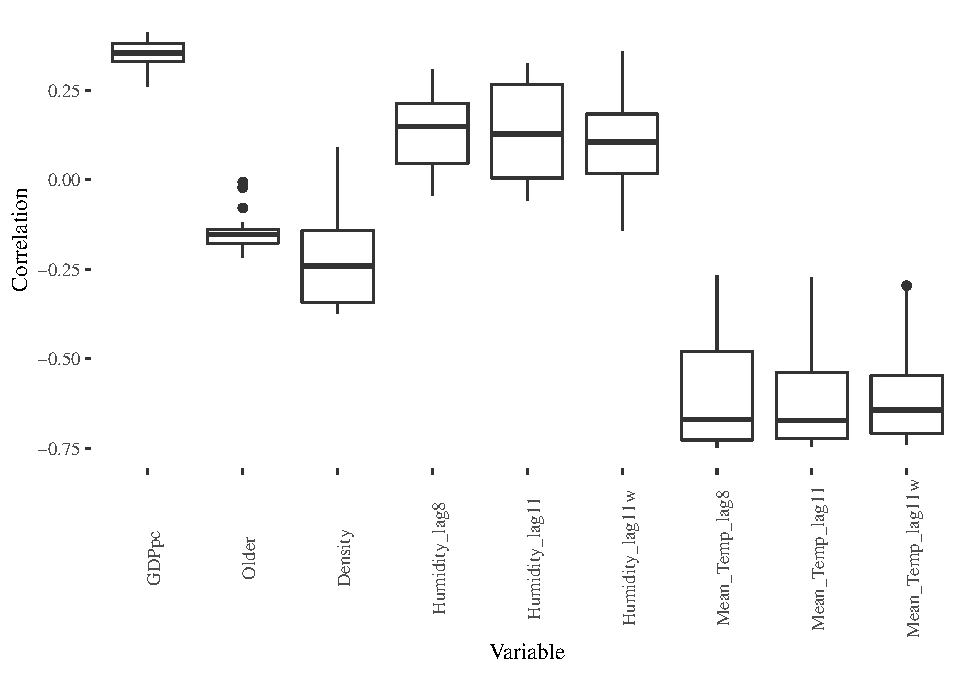
\includegraphics{Climatic-Correlates-of-COVID19-Spain_files/figure-latex/daily-correlations-1.pdf}
\caption{\label{fig:daily-correlations}Distribution of daily
correlations of the independent variables with daily incidence of
COVID-19 (all variables have been log-transformed)}
\end{figure}

\hypertarget{sur-systems}{%
\subsection{SUR Systems}\label{sur-systems}}

The goodness of fit of the three systems of equations is shown in Figure
\ref{fig:goodness-of-fit}.

\begin{figure}
\centering
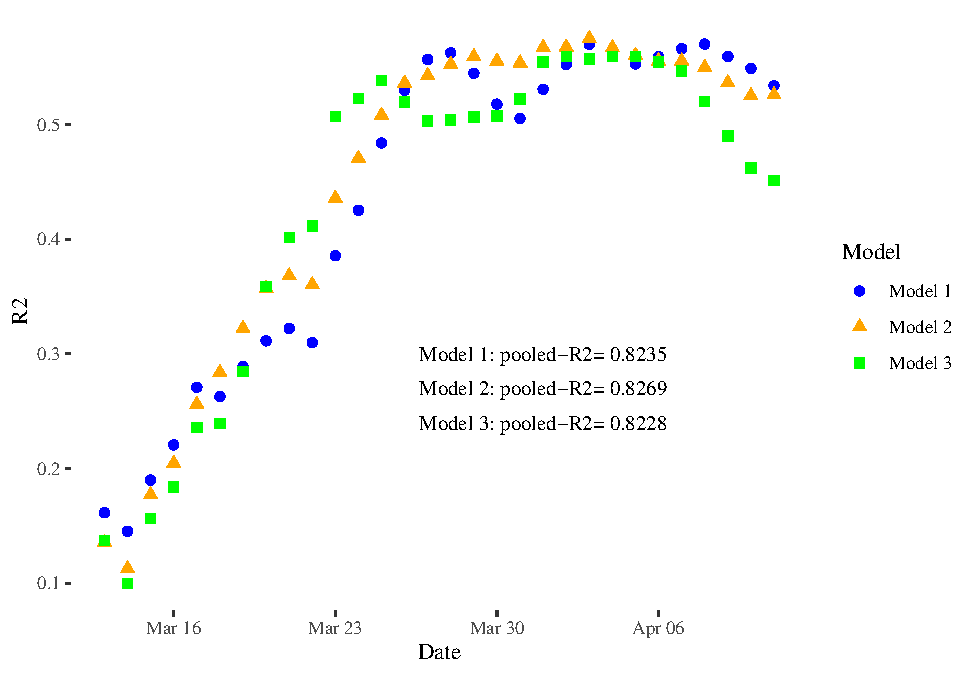
\includegraphics{Climatic-Correlates-of-COVID19-Spain_files/figure-latex/goodness-of-fit-1.pdf}
\caption{\label{fig:goodness-of-fit} Goodness of fit of the SUR systems:
by date and pooled}
\end{figure}

\hypertarget{discussion}{%
\section{Discussion}\label{discussion}}

Possibly do some simulations with the model.

\hypertarget{concluding-remarks}{%
\section{Concluding Remarks}\label{concluding-remarks}}

More words go here.

\hypertarget{acknowledgments}{%
\section*{Acknowledgments}\label{acknowledgments}}
\addcontentsline{toc}{section}{Acknowledgments}

Add acknowledgments as appropriate in final draft.

The following \texttt{R} packages were used in the course of this
investigation and the authors wish to acknowledge their developers:
\texttt{aemet} {[}{]}, \texttt{ggthemes} (Arnold, 2019),
\texttt{gridExtra} (Auguie, 2017), \texttt{kableExtra} (Zhu, 2019),
\texttt{knitr} (Xie, 2015, 2014), \texttt{lubridate} (Grolemund and
Wickham, 2011), \texttt{plm} (Millo, 2017), \texttt{rticles} (Allaire et
al., 2020), \texttt{sf} (Pebesma, 2018), \texttt{spdep} (Bivand et al.,
2013), spsur (Angulo et al., 2020) \texttt{tidyverse} (Wickham et al.,
2019), \texttt{units} (Pebesma et al., 2016).

\hypertarget{references}{%
\section*{References}\label{references}}
\addcontentsline{toc}{section}{References}

\hypertarget{refs}{}
\leavevmode\hypertarget{ref-Allaire2020}{}%
Allaire, J., Xie, Y., R Foundation, Wickham, H., Journal of Statistical
Software, Vaidyanathan, R., Association for Computing Machinery,
Boettiger, C., Elsevier, Broman, K., Mueller, K., Quast, B., Pruim, R.,
Marwick, B., Wickham, C., Keyes, O., Yu, M., Emaasit, D., Onkelinx, T.,
Gasparini, A., Desautels, M.-A., Leutnant, D., MDPI, Taylor and Francis,
Ögreden, O., Hance, D., Nüst, D., Uvesten, P., Campitelli, E.,
Muschelli, J., Kamvar, Z.N., Ross, N., Cannoodt, R., Luguern, D.,
Kaplan, D.M., 2020. Rticles: Article formats for r markdown.

\leavevmode\hypertarget{ref-Angulo2020spsur}{}%
Angulo, A., Lopez, F.A., Minguez, R., Mur, J., 2020. Spsur: Spatial
seemingly unrelated regression models.

\leavevmode\hypertarget{ref-Arnold2019}{}%
Arnold, J.B., 2019. Ggthemes: Extra themes, scales and geoms for
'ggplot2'.

\leavevmode\hypertarget{ref-Auguie2017gridextra}{}%
Auguie, B., 2017. GridExtra: Miscellaneous functions for "grid"
graphics.

\leavevmode\hypertarget{ref-Bivand2013}{}%
Bivand, R.S., Pebesma, E., Gomez-Rubio, V., 2013. Applied spatial data
analysis with R, second edition. Springer, NY.

\leavevmode\hypertarget{ref-Casanova2010effects}{}%
Casanova, L.M., Jeon, S., Rutala, W.A., Weber, D.J., Sobsey, M.D., 2010.
Effects of air temperature and relative humidity on coronavirus survival
on surfaces. Appl. Environ. Microbiol. 76, 2712--2717.

\leavevmode\hypertarget{ref-Chan2011effects}{}%
Chan, K., Peiris, J., Lam, S., Poon, L., Yuen, K., Seto, W., 2011. The
effects of temperature and relative humidity on the viability of the
sars coronavirus. Advances in virology 2011.

\leavevmode\hypertarget{ref-Fernandes2020economic}{}%
Fernandes, N., 2020. Economic effects of coronavirus outbreak (covid-19)
on the world economy. Available at SSRN 3557504.

\leavevmode\hypertarget{ref-Gong2020balance}{}%
Gong, B., Zhang, S., Yuan, L., Chen, K.Z., 2020. A balance act:
Minimizing economic loss while controlling novel coronavirus pneumonia.
Journal of Chinese Governance 1--20.

\leavevmode\hypertarget{ref-Grolemund2011dates}{}%
Grolemund, G., Wickham, H., 2011. Dates and times made easy with
lubridate. Journal of Statistical Software 40, 1--25.

\leavevmode\hypertarget{ref-Jaakkola2014decline}{}%
Jaakkola, K., Saukkoriipi, A., Jokelainen, J., Juvonen, R., Kauppila,
J., Vainio, O., Ziegler, T., Rönkkö, E., Jaakkola, J.J., Ikäheimo, T.M.,
2014. Decline in temperature and humidity increases the occurrence of
influenza in cold climate. Environmental Health 13, 22.

\leavevmode\hypertarget{ref-Kissler2020projecting}{}%
Kissler, S.M., Tedijanto, C., Goldstein, E., Grad, Y.H., Lipsitch, M.,
2020. Projecting the transmission dynamics of sars-cov-2 through the
postpandemic period. Science eabb5793.
doi:\href{https://doi.org/10.1126/science.abb5793}{10.1126/science.abb5793}

\leavevmode\hypertarget{ref-Kudo2019low}{}%
Kudo, E., Song, E., Yockey, L.J., Rakib, T., Wong, P.W., Homer, R.J.,
Iwasaki, A., 2019. Low ambient humidity impairs barrier function and
innate resistance against influenza infection. Proceedings of the
National Academy of Sciences 116, 10905--10910.

\leavevmode\hypertarget{ref-Lancastle2020impact}{}%
Lancastle, N.M., 2020. Is the impact of social distancing on coronavirus
growth rates effective across different settings? A non-parametric and
local regression approach to test and compare the growth rate. medRxiv.

\leavevmode\hypertarget{ref-Luo2020how}{}%
Luo, S., Tsang, K.P., 2020. How much of china and world gdp has the
coronavirus reduced? Available at SSRN 3543760.

\leavevmode\hypertarget{ref-Makinen2009cold}{}%
Mäkainen, T.M., Juvonen, R., Jokelainen, J., Harju, T.H., Peitso, A.,
Bloigu, A., Silvennoinen-Kassinen, S., Leinonen, M., Hassi, J., 2009.
Cold temperature and low humidity are associated with increased
occurrence of respiratory tract infections. Respiratory medicine 103,
456--462.

\leavevmode\hypertarget{ref-Millo2017robust}{}%
Millo, G., 2017. Robust standard error estimators for panel models: A
unifying approach. Journal of Statistical Software 82, 1--27.
doi:\href{https://doi.org/10.18637/jss.v082.i03}{10.18637/jss.v082.i03}

\leavevmode\hypertarget{ref-Pebesma2018}{}%
Pebesma, E., 2018. Simple Features for R: Standardized Support for
Spatial Vector Data. The R Journal 10, 439--446.
doi:\href{https://doi.org/10.32614/RJ-2018-009}{10.32614/RJ-2018-009}

\leavevmode\hypertarget{ref-Pebesma2016}{}%
Pebesma, E., Mailund, T., Hiebert, J., 2016. Measurement units in R. R
Journal 8, 486--494.
doi:\href{https://doi.org/10.32614/RJ-2016-061}{10.32614/RJ-2016-061}

\leavevmode\hypertarget{ref-Wickham2019}{}%
Wickham, H., Averick, M., Bryan, J., Chang, W., McGowan, L.D., François,
R., Grolemund, G., Hayes, A., Henry, L., Hester, J., Kuhn, M., Pedersen,
T.L., Miller, E., Bache, S.M., Müller, K., Ooms, J., Robinson, D.,
Seidel, D.P., Spinu, V., Takahashi, K., Vaughan, D., Wilke, C., Woo, K.,
Yutani, H., 2019. Welcome to the tidyverse. Journal of Open Source
Software 4, 1686.
doi:\href{https://doi.org/10.21105/joss.01686}{10.21105/joss.01686}

\leavevmode\hypertarget{ref-Xie2014}{}%
Xie, Y., 2014. Knitr: A comprehensive tool for reproducible research in
R, in: Stodden, V., Leisch, F., Peng, R.D. (Eds.), Implementing
Reproducible Computational Research. Chapman; Hall/CRC.

\leavevmode\hypertarget{ref-Xie2015}{}%
Xie, Y., 2015. Dynamic documents with R and knitr, 2nd ed. Chapman;
Hall/CRC, Boca Raton, Florida.

\leavevmode\hypertarget{ref-Zhu2019}{}%
Zhu, H., 2019. KableExtra: Construct complex table with 'kable' and pipe
syntax.


\end{document}


